\documentclass[20pt]{article}
\usepackage{graphicx}
\begin{document}

\title{Networks Assignment}
\author
{
	{Prashant A, Gopinath S\\
	2011103043, 2011103031}
}
\maketitle
\section{Tier 1 and Tier 2 ISPs}
\\\textbf{\emph{Tier 1}}
Although there is no authority that defines tiers of networks participating in the Internet, the most common definition of a tier 1 network is one that can reach every other network on the Internet without purchasing IP transit or paying settlements.
\\Companies:
\begin{enumerate}
	\\\item{AT&T}
	\\\item{Verizon}
	\\\item{Sprint (Softbank Broadband)}
	\\\item{Century Link (Qwest)}
	\\\item{Level 3 (with Global Crossing now)}
	\\\item{NTT/Verio}
	\\\item{Cogent (maybe?)}
	\\\item{Bharti}
	\\\item{Reliance}
	\\\item{Tata}
	\\\item{VSNL}
\end{enumerate}
\\\textbf{\emph{Tier 2}}
\\A network that peers with some networks, but still purchases IP transit or pays settlements to reach at least some portion of the Internet.
\\Companies:
\begin{enumerate}
	\\\item{Headstrong} \\\item{Microland} \\\item{MindTree} \\\item{MphasiS }\\\item{Sonata Software. }
\end{enumerate}

\\\textbf{\emph{Tier 3}}
\\A network that solely purchases transit from other networks to reach the Internet.
Companies:
\begin{enumerate}
	\\\item{CCS out of Austin, Texas}
	\\\item{ Rt. 66 Internet in New Mexico }
	\\\item{Quik Internet in New Jersey }
\end{enumerate}
\\\\Source : 
\url{https://secure.dslreports.com/forum/r24946459-What-is-a-Tier-1-2-and-3-service-provider-}
\section{What is RFC?}
 
RFC is ``Request For Comment''
\\A RFC is authored by engineers and computer scientists in the form of a memorandum describing methods, behaviors, research, or innovations applicable to the working of the Internet and Internet-connected systems.
\\\\Source: \url{http://www.internetslang.com/RFC-meaning-definition.asp}
\section{What is a packet sniffer?}
A packet sniffer simply captures all of the packets of data that pass through a given network interface. Typically, the packet sniffer would only capture packets that were intended for the machine in question. However, if placed into promiscuous mode, the packet sniffer is also capable of capturing ALL packets traversing the network regardless of destination. 
\\\\Source: \url{http://netsecurity.about.com/cs/hackertools/a/aa121403.htm}
\section{Nslookup for 5 hosts}
\begin{figure}[ht!]
	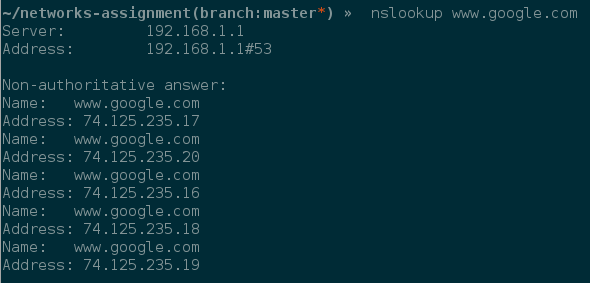
\includegraphics[width=90mm]{1.png}
	\caption{google}
	\label{overflow}
\end{figure}
\begin{figure}[ht!]
	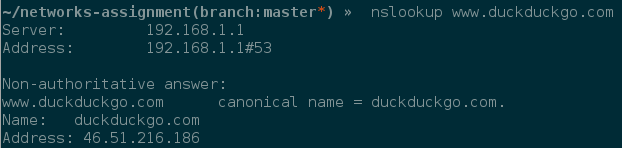
\includegraphics[width=90mm]{2.png}
	\caption{duckduckgo}
	\label{overflow}
\end{figure}
\begin{figure}[ht!]
	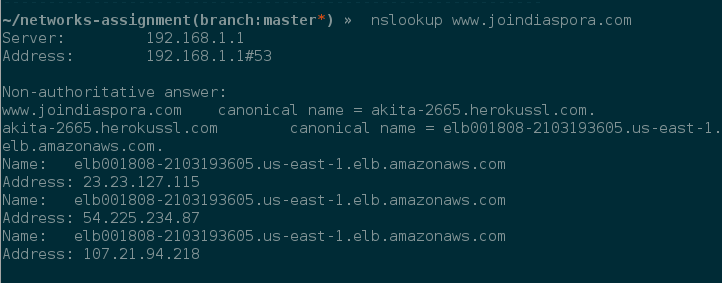
\includegraphics[width=90mm]{3.png}
	\caption{joindiaspora}
	\label{overflow}
\end{figure}
\begin{figure}[ht!]
	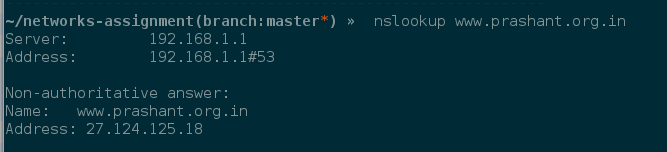
\includegraphics[width=90mm]{4.png}
	\caption{My site}
	\label{overflow}
\end{figure}

\begin{figure}[ht!]
	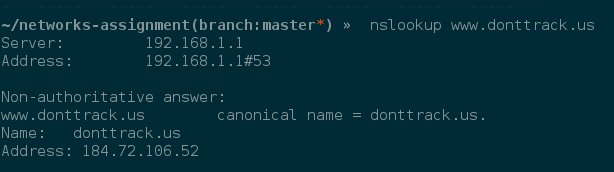
\includegraphics[width=90mm]{5.png}
	\caption{dont track us}
	\label{overflow}
\end{figure}
\end{document}
